\documentclass[conference]{IEEEtran}
\IEEEoverridecommandlockouts
%\documentclass[a4paper,12pt]{article}

%vorgegeben
\usepackage{balance}
\usepackage{graphicx}
\usepackage{booktabs}
\usepackage{relsize}
\usepackage{pgfplots}
\usepackage{tabularx}
\usepackage{gensymb}
\usepackage{caption}
\usepackage{listings}
\usepackage{babel}
\usepackage{siunitx}
\usepackage{url}
\usepackage{subcaption}
\usepackage{comment}
\usepackage{tikz}

%packages to eneble new font
\usepackage{fontspec}
\setmainfont{Myriad Pro}
%\setsansfont{Myriad Pro}
%\newfontfamily\computermodern{Computer Modern}
%\setsansfont{Latin Modern}

%no Idea why I have these
\usepackage[utf8]{inputenc}
\usepackage{amsmath}
\usepackage{hyperref}

%to enble captions vor the graphics
\usepackage{caption}

\usepackage{array} %enebels tabular

%neue pacages vom neuen Template
\usepackage{cite}
\usepackage{amssymb,amsfonts} %hier vorher: \usepackage{amsmath,amssymb,amsfonts}
\usepackage{algorithmic}
\usepackage{textcomp}
\usepackage{xcolor}
\usepackage{epstopdf}
\usepackage{multirow}
\usepackage{blindtext}
\pgfplotsset{compat=1.18}
\title{\textbf{Shortpaper:} IoT-NDN: An IoT Architecture via Named Data
Netwoking (NDN)\\}
\author{Leonard Boetefuer}
\date{\today}


\begin{document}

\maketitle

\begin{abstract}
als Leztes
\end{abstract}

\section{Introduction}
als vorleztes
\section{Related Work}
XYZTEST2
\section{Analysis of IoT and NDN}
This section will talk about the limitations of IoT devices
 and the challenges of the current Internet architecture.
\subsection{Challanges of the IoT}
1) \textbf{The connectivity of IoT devices:}
Currently, IoT devices use a server-client or host-to-host connection, 
neither is scalable enough for a billion devices.
%The server-client architecture has a bottleneck in the server.
%was für ein Bottlenck (nur ein server kann durch anfragen überlastet werden)
In the host-host architecture, every host has to communicate with every other host, 
resulting in exponential resource consumption.
%The server-client and the host-to-host model both need IP addresses for every single device, which is not possible with a billion devices.
%NDN solves the IP shortage and it is de-central helps with the bottleneck
%100

2) \textbf{Technological Standards:}
The current standards are inadequate for network protocols, communication protocols, 
and data aggregation. They lead to inefficient caching and aggregation. 
In addition, mobility protocols are needed to mitigate the effect of a connection loss. 
%vielleicht schöner und/oder kürzer
%97

3) \textbf{Mobility:}
IoT systems that use mobile devices need to note, that devices are numerous and technologically diverse, 
and consumer reliance is increasing. 
% über 90


4) \textbf{Complexity and Integration Issues:}
IoT systems comprise many unique Application Programming Interfaces (APIs), protocols, and platforms. 
%APIs expeccially are not desined with the resource limitations of IoT devices in mind. 
% maybe add that later
The integration of technologies into the system is very complicated 
due to all the different combinations. 
This system should consider the resource limitation of its components.
%100

%AB HIER BEGINNT B

\subsection{NDN for the IoT}
%erstes mal NDN erwähnt (auser intorduction)

1) \textbf{NDN Packet Length:}
Packages in NDN are not bound to a specific length, 
which allows expansion of further protocols by adding or subtracting from the overhead.
IoT devices are limited in memory, resulting in small packages with a necessity of a small overhead.
%100



%Packages in NDN are not bound to a specific length. This is helpful to expand further protocols by adding or subtracting from the overhead.
%IoT devices will send only small packages; because of the limited resources in memory, resulting in the necessity of a small overhead.

%The overhead must be kept small because the information proportion of small packets is much more influenced by a large overhead.
%to many packages will drain energy and put strain on the network.
%Quelle 16 (nicht benutzt)
2) \textbf{Caching in IoT/NDN:}
IoT devices have too little memory for efficient caching, resulting in 
higher unnecessary package flow and a reduction in data freshness.
The solution is in-network caching, a feature of NDN; that allows 
% wie wird in-network caching grob umgesetzt?

%ALTER TEXT
%Data freshness and reduced unnecessary package flow, is achieved by integrating an in-network cache, which is a feature of NDN.
%To keep the data up to date and reduce unnecessary package flow, we need to integrate caches into the system. 
%The problem is that the small devices don't have enough memory to keep an efficient cache. 
%The solution is to use in-network caching, a feature of NDN.
%ganz kurz in-network caching erklären.
%Quelle 11
%Even a small cache will dramatically increase the data availability [11].
%Quelle 2


3) \textbf{Data Aggregation in Wireless Networks:}
If a user's query requests data that includes multiple packages, 
each package will be requested separately (excluding the others); 
resulting in a greater overhead and more unnecessary package flow. 
The new system should fix the request problem.
%97

4) \textbf{Naming Problems in Wireless Networks:}
NDN supports name-centric services [17], which facilitates access without knowing their location. There is still a need to automate naming conventions, because of the size of the Networks. These Names should be kept short to minimize storage usage. 
%Quelle 18 (3 mal)


5) \textbf{Routing Scalability in NDN:}
In NDN routing is managed by names, instead of usual number based systems. The scalability of routing is important to facilitate a large network.
% Da fehlt was mach das vielleicht später
% Quelle 19 und 20

\section{Architecture of IoT-NDN System}

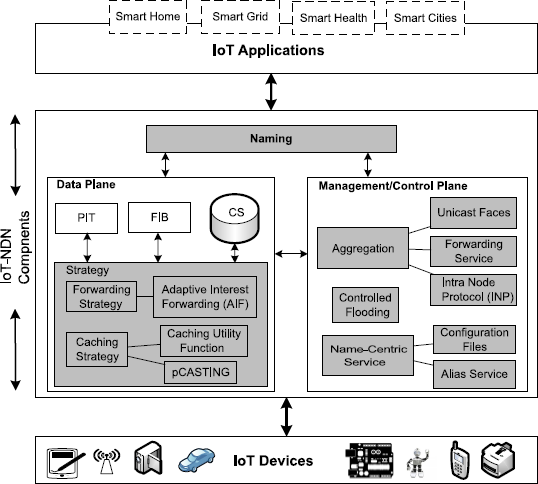
\includegraphics[width=0.3\textwidth]{IoT-NDN_System_architecture_and_its_components.png}\\
IoT-NDN has three main components. The \textbf{naming} component is made up of naming schemes and structure for wireless networks.
The \textbf{Management and control plane} is made up of Unicast Faces; Forwardinng Services Intra Node Protocol, Controlled Flooding, Configuartion and Alias services. %aus Paper Zitiert. Vielleicht über graphic kürzen.
The \textbf{dataplan component} is made up of the caching and forwarding strategies.
The IoT-NDN components are responsible for packages, caching, strategies and other. %grey component?
Devices in the IoT-NDN architecture have three tables: CS, PIT and FIB.
%Quelle 2
NDN solves issues many issues discussed in III. For more information, see graphic 2.

%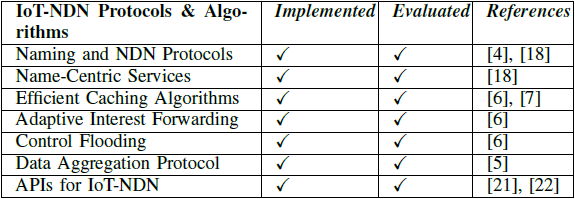
\includegraphics[width=0.3\textwidth]{IMPLEMENTED_AND_TESTED_PROTOCOLS_AND_ALGORITHMS_IN_IOT-NDN.png}\\
{\tiny
\begin{tabular}{ | m{2,0cm} | m{1,5cm}| m{1,5cm} |  m{1,5cm} |} 
  \hline
  \textbf{IoT-NDN Protocols \& Algorithms}& \textbf{Implementation} & \textbf{Evaluation} & \textbf{References} \\ 
  \hline
  Naming and NDN Protocols & \checkmark & \checkmark & \cite{b4},\cite{b18} \\ 
  \hline
  Name-Centric Services & \checkmark & \checkmark & \cite{b18}\\ 
  \hline
  Efficient Caching Algorithm & \checkmark & \checkmark & \cite{b6},\cite{b7} \\ 
  \hline
  Adaptive Internet Forwarding & \checkmark & \checkmark & \cite{b6} \\ 
  \hline
  Control Flooding & \checkmark & \checkmark & \cite{b6} \\ 
  \hline
  Data Aggregation Protocol & \checkmark & \checkmark & \cite{b5} \\ 
  \hline
  APIs for IoT-NDN & \checkmark & \checkmark & \cite{b21},\cite{b22} \\ 
  \hline

\end{tabular}

}

\subsection{Naming}
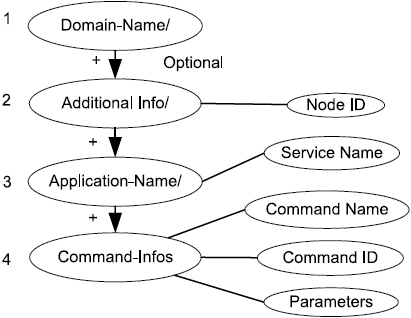
\includegraphics[width=0.3\textwidth]{Name_Structure_of_the_suggested_Approach.png}\\
In IoT-NDN the structure in which data is addressed is hierarchical. As shown in graphic 3. 
The first component is a global Domain-Name. 
The second is optional and, if used, stores additional information, like node ID.
The third component contains the application and service name.
The fourth component contains information about the command name, command ID and additional parameters.
The marker component would be the additional fifth component of the name, specific to IoT-NDN.
It contains application, service or device resource information.
The marker component can 
%was kann sie und wofür braucht man sie?

\subsection{Managment and Control Plane}
1) \textbf{Aggregation:} Data aggregation is improtant to reduce the memory size of CS and the energy consumption, by combining similar information into one package. Data aggregation is achieved by three components. The components are: Forwarding Service, Unicast Faces and Intra Node Protocol (INP); they are explained in greater detail in [5]. 
%erkläre Unicast Faces.#
%was ist radio layer (die sicherungsschicht?)
Unicast Face needs every package, in the radio layer, to include the source and destination address. 
When a device receives a package, it will build a connection to the sender of the package. 
This enables devices to learn their neighbors. %? stimmt das
If a connection is lost, for this connection allocated resources will be released. 
%später noch ergänzen

2) \textbf{Controlled Flooding:}
IoT-devices are unreliable in power or connectivity. % 70%sicher
As a result the Forwarding Information Base (FIB) tables wont usually be populated in advance by routing information. %ziemlich eins zu eins übernommen
Packages will transfer from one device to another and to mitigate flooding, controlled flooding is used.
To reduce overhead and redundancy, devices will delay sending out packages. This time can be random or based on network topology.
While a package is delayed and arrives  again at the same device, the package is not send out twice. 
The path is selected
%MUSS NOCH PATH SELECTION MACHEN

3) \textbf{Name-Centric Services:}
The use of a Gateway enables IoT-Devices to be reachable from any internet device. 
The Gateway allows via protocol conversion wireless and wired connection. %falsch durch formulierung
The Gateway provides all important configurations of names and  IoT-NDN devices. Services on the gateway can be implemented as IoT-NDN applications and communicate to each other via the IoT-NDN deamon and face. %ziemlich eins zu eins übernommen.
To reduce the workload on the IoT devices the gateway will use aliases, that are shorter, to reduce the size  of the packages.
Names form the recived  the internet will be mapped to names used in the Iot-NDN network.

\subsection{Data Plane}
1) \textbf{Strategy-In-Network Caching:} 
The CS is a caching place in IoT-NDN devices, unlike Routers in the IP protocol it can send cached packages more than once.
If receives a package request it, will first check the CS, by checking of matching prefixs. %the it will be send out
This is done because the same data will probably be requested many times in IoT-NDN networks.
The standard replacement strategy is LRU, but others can be implemented. %LFU und randome auch gut mit quelle 7 und 26
Iot-NDN devices have a special probabilistic CAching STrategy (pCASTING), that considers data freshness and the charge and storage of devices. This strategy is used %among other things
when a data package with a matching PIT is received by a device.
% vieelicht mehr über pCasting, dann aber auch quelle 7 zitiern

2) \textbf{Strategy-Forwarding:}
The forwarding Path is selected from the FIB to forward Interest packets, by the forwarding strategy component. %ziemlich 1 zu 1 nicht gut
by remembering the number of unsatisfied Interests, the forwarding strategy could be used to control the traffic. %auch 1 zu 1
The forwarding component the path of the Interest by using data such as delay and throughput. % 1. wieder nah dran 2. vielleicht "Interest package" 3. funkitoniert path oder doch wie im paper?
Forwarding steps on devices are supported by IoT-NDN and the forwarding strategy allows the requesting of lost packages in network, by using its metrics. % fehlt "name loockup"
These metrics can be used to study the performance of every face.
%nicht gut zu schwammig
Fining missing packages can also be achieved with the InterestLifeTime parameter. For more info see \cite{b6}


\section{Conclusion}
First, the paper highlights the problems of IoT if implemented in IP. 
%Then it examines cache mechanisms, data aggregation and naming in wireless networks.
NDN is not built with resource constrained devises in mind. This paper names the problems and solutions of integrating NDN into IoT.
The result Iot-NDN is a new type network that includes communication and data access, based on names.








\section{References}
\begin{thebibliography}{00}
    \bibitem{b1}M. A. Heil, "IoT-NDN: An IoT Architecture via Named Data
    Netwoking (NDN)" in Software Embedded System Department
    Euroimmun AG, a PerkinElmer Company
    \bibitem{b4} Z. Ren, M. Hail, and H. Hellbruck, “Ccn-wsn - a lightweight, flexible
    content-centric networking protocol for wireless sensor networks,” in
    Intelligent Sensors, Sensor Networks and Information Processing, 2013.
    \bibitem{b5} T. Teubler, M. A. M. Hail, and H. Hellbr¨uck, “Efficient Data Aggregation
    with CCNx in Wireless Sensor Networks,” in 19th EUNICE Workshop
    on Advances in Communication Networking (EUNICE 2013), Germany.
    \bibitem{b6}M. A. Hail, M. Amadeo, A. Molinaro, and S. Fischer, “On the performance
    of caching and forwarding in information centric networking for
    the iot,” in 13th International Conference on Wired and Wireless Internet
    Communications, April 2015.
    \bibitem{b7}——, “Caching in named data networking for the wireless internet
    of things,” in Recent Advances in Internet of Things (RIoT), 2015
    International Conference on, April 2015, pp. 1–6.
    \bibitem{b18}T. Teubler, M. A. M. Hail, and H. Hellbr¨uck, “A solution for the
    naming problem for name-centric services,” in Wired/Wireless Internet
    Communications, A. Mellouk, S. Fowler, S. Hoceini, and B. Daachi,
    Eds. Cham: Springer International Publishing, 2014, pp. 214–227.
    \bibitem{b21}S. Ebers, M. A. Hail, S. Fischer, and H. Hellbr¨uck, “Api for data
    dissemination protocols - evaluation with autocast,” in The Third World
    Congress on Nature and Biologically Inspired Computing (NaBIC 2011).
    Salamanca, Spain: IEEE, Oct. 2011, pp. 534–539.
    \bibitem{b22}M. A. Hail and S. Fischer, “Flexible API for IoT Services with Named
    Data Networking,” in 2016 IEEE International Conference on Emerging
    Technologies and Innovative Business Practices for the Transformation
    of Societies (IEEE EmergiTech 2016), Mauritius, Mauritius, Aug 2016.
    \end{thebibliography}
\end{document}